\documentclass[12pt]{article}
\usepackage[english]{babel}
\usepackage{hyperref}
\usepackage{natbib}
\usepackage{url}
\usepackage[utf8x]{inputenc}
\usepackage{amsmath}
\usepackage{graphicx}
\graphicspath{{images/}}
\usepackage{parskip}
\usepackage{fancyhdr}
\usepackage{vmargin}
\usepackage{enumitem}
\usepackage{tcolorbox}
\usepackage{pdfpages}
\usepackage{tikz}
\usepackage{listings}
\lstset{frame=tb,
  language=Bash,
  aboveskip=3mm,
  belowskip=3mm,
  showstringspaces=false,
  columns=flexible,
  basicstyle={\small\ttfamily},
  numbers=none,
  numberstyle=\tiny\color{gray},
  keywordstyle=\color{blue},
  commentstyle=\color{dkgreen},
  stringstyle=\color{mauve},
  breaklines=true,
  breakatwhitespace=true,
  tabsize=3
}
\usepackage{minted}
% CODIGO
\usepackage{listings}
\usepackage{color}
\usepackage{mdframed}
\usepackage{xcolor}
\usepackage{fancyvrb}
\definecolor{bg}{rgb}{0.95,0.95,0.95}
\setmarginsrb{3 cm}{2.5 cm}{3 cm}{2.5 cm}{1 cm}{1.5 cm}{1 cm}{1.5 cm}
\usepackage{pdfpages}
\usepackage{drawstack}
\title{Trabajo Práctico 2}						% Title
\author{Bach, Montes, Luizaga y La Torre}			% Author
\date{}											% Date

\makeatletter
\let\thetitle\@title
\let\theauthor\@author
\let\thedate\@date
\makeatother

\pagestyle{fancy}
\fancyhf{}
\rhead{\theauthor}
\lhead{\thetitle}
\cfoot{\thepage}

\lstdefinestyle{customasm}{
  belowcaptionskip=1\baselineskip,
  frame=L,
  xleftmargin=\parindent,
  language=[x86masm]Assembler,
  basicstyle=\footnotesize\ttfamily,
  commentstyle=\itshape\color{purple!40!black},
}

\lstdefinestyle{BASH}{
    backgroundcolor=\color{black},
    basicstyle=\scriptsize\color{white}\ttfamily,
    frame=none
}

\begin{document}

%%%%%%%%%%%%%%%%%%%%%%%%%%%%%%%%%%%%%%%%%%%%%%%%%%%%%%%%%%%%%%%%%%%%%%%%%%%%%%%%%%%%%%%%%

\begin{titlepage}
	\centering
    \vspace*{-5 cm}
    
\includegraphics[scale = 1]{imgs/fiuba.png}\\[1.0 cm]	% University Logo
    \textsc{\LARGE Organización de Datos}\\[0.5 cm]	% University Name
	\textsc{\Large Competencia Machine Learning - Real or Not? NLP with Disaster Tweets}\\[2 cm]
	\textsc{Repositorio: }
	\url{https://github.com/GastonMontes/1ro-2020-7506-TP2}\\[0.5 cm]
	\textsc{Competicion: }
	\url{https://www.kaggle.com/c/nlp-getting-started}\\[0.5 cm]
	\rule{\linewidth}{0.2 mm} \\[0.4 cm]
	{ \huge \bfseries \thetitle}\\
	\rule{\linewidth}{0.2 mm} \\[1.5 cm]
	\textsc{Grupo Pyrañas}\\[1 cm]
	\begin{minipage}{0.4\textwidth}
		\begin{flushleft} \large
			\emph{Integrantes}\\
			Gastón Montes\\
            Gabriel La Torre\\
        	Ricardo Luizaga\\
        	Alan Bach\\
        \end{flushleft}
	\end{minipage}~
    \begin{minipage}{0.18\textwidth}
		\begin{center} \large
          \emph{Padrón} \\ 
          89397\\
          87796\\
          87528\\
          91440
        \end{center}
	\end{minipage}~\\[2 cm]
    \normalsize{1er. Cuatrimestre de 2020} \\
\end{titlepage}

%%%%%%%%%%%%%%%%%%%%%%%%%%%%%%%%%%%%%%%%%%%%%%%%%%%%%%%%%%%%%%%%%%%%%%%%%%%%%%%%%%%%%%%%%

\tableofcontents
\pagebreak

%%%%%%%%%%%%%%%%%%%%%%%%%%%%%%%%%%%%%%%%%%%%%%%%%%%%%%%%%%%%%%%%%%%%%%%%%%%%%%%%%%%%%%%%%
\newpage
\section{Introducción}

%%%%%%%%%%%%%%%%%%%%%%%%%%%%%%%%%%%%%%%%%%%%%%%%%%%%%%%%%%%%%%%%%%%%%%%%%%%%%%%%%%%%%%%%%
\textbf{
El presente trabajo práctico consta de una competencia de machine learning en donde el grupo deberá utilizar diferentes algoritmos o ensambles de algoritmos presentados en clases con el fin de predecir si un Tweet del set de test pertenece a un desastre real o no.
Para este fin se cuenta con dos sets de datos: el train.csv y el test.csv. Se deberá entrenar y validar los diferentes algoritmos utilizando el set de train mientras que se deberá realizar las predicciones sobre el set de test.
Este problema de machine learning es un problema de clasificación ya que se debe predecir si un tweet pertenece a una clase o a la otra: si el tweet es real o no.
}

\subsection{Introducción teórica}
A continuación se detallan algunos conceptos básicos o algoritmos de machine learning vistos en clase y que se aplicarán en los algoritmos de machine learning a la hora de realizar la clasificación.

\subsection{Entrenamiento}
El entrenamiento de un modelo de machine learning es un problema de optimización que consiste en buscar los parámetros que maximizan/minimizan la clasificación.
Es el proceso que más tiempo y recursos consume en general en los modelos de machine learning y varían dependiendo el modelo a utilizar.
Una vez entrenado el modelo, el mismo queda representado por sus parámetros.


\subsection{Errores}
A un procesador arriban instrucciones siguiendo una distribución exponencial con una tasa de $250$ instrucciones por microsegundo.

\subsubsection{Error de entrenamiento}
Es el error que tenemos al realizar el entrenamiento del algoritmo y su posterior validación.

\subsubsection{Error de test}
Es el error que obtenemos al realizar el entrenamiento del algoritmo y luego realizar predicciones sobre un nuevo set de datos (set de test).
En otras palabras, es el error de generalización de nuestro algoritmo.


\subsection{Underfitting}
El underfitting sucede cuando el algoritmo tiene un error de entrenamiento alto, es decir, el algoritmo no ajusta correctamente a nuestro set de entrenamiento.
El modelo carece de capacidad expresiva, no tiene suficientes grados de libertad o complejidad.
Cuando se tiene underfitting es una buena idea cambiar de modelo a uno de mayor complejidad.


\subsection{Overfitting}
El overfitting es cuando nuestro modelo ajusta realmente muy bien a nuestro set de entrenamiento, pero a la hora de generalizar no produce resultados buenos. Es decir, el error de entrenamiento es bajo y el error de test es alto.
El modelo generaliza mal debido a que se sobreentrena y se dice que se "memoriza" el set de entrenamiento.


\subsection{Forward Selection}
Al realizar una clasificación no todos los features son adecuados para clasificar. Mediante forward selection se filtran aquellos features que impactan positivamente en la clasificación: se realiza una primera clasificación sin features y en cada paso se agrega un feature a la clasificación, si el resultado de la clasificación mejora agregamos el feature, sino lo descartamos.


\subsection{Backward Selection}
La idea es idéntica a forward selection con la diferencia que en backward selection se empieza con todos los features y en cada iteración se elimina uno de los features, si el resultado de la clasificación mejora entonces eliminamos la feature, sino la de dejamos.

\subsection{Grid Search}
Los diferentes algoritmos de machine learning que utilizamos presentan hiper-parámetros que pueden ser valores discretos o continuos y a su vez pueden ser finitos o no.
Con grid search se intenta buscar los hiper-parámetros óptimos de la siguiente manera: se prueban todas las combinaciones posibles para los hiper-parámetros y se elige aquella que dió los mejores resultados.

\subsection{Random Search}
Al igual que en grid search, con este algoritmo se intentan determinar los hiper-parámetros óptimos para el algoritmo de machine learning a utilizar. En este caso se prueban k combinaciones posibles de los hiper-parámetros de forma aleatoria y se queda con la mejor combinación encontrada.
Cabe destacar que con random search no se encuentran los parámetros óptimos pero a su vez se puede calcular el tiempo invertido en la búsqueda de los hiper-parámetros.

\subsection{Cross Validation}
Al entrenar el algoritmo se utiliza el set de entrenamiento para esto, sin embargo, se debe tener una idea de si el algoritmo está prediciendo bien o mal. Para realizar este chequeo se crea un set de validación a partir del set de entrenamiento, se entrena el modelo con el set de entrenamiento y luego se lo valida con este sub-set de validación.
En cross validation se particiona el set de entrenamiento en k bloques, se selecciona uno de estos bloques como bloque de validación, se entrena el algoritmo con los bloques restantes y luego se valida con el bloque seleccionado como de validación. Cada bloque debe actuar como bloque de validación.
Este algoritmo está implementado en la mayoría de las librerías de machine learning.


\subsection{Bootstrapping}
Este algoritmo consiste en tomar una muestra del set de entrenamiento del mismo tamaño que el set de entrenamiento con reemplazo, se entrena el algoritmo con n bootstraps distintos obteniendo así n clasificadores distintos.


\subsection{Bagging}
Bagging es una técnica muy utilizada con el fin de no caer en overfitting.
Consiste en aplicar n veces el mismo algoritmo y luego promediar el resultado.
Se generan n sets de entrenamientos distintos a partir del set de entrenamiento dado (Con Bootstrapping por ejemplo), se aplica el algoritmo a esos n set de entrenamientos distintos y luego se promedian los resultados.



%%%%%%%%%%%%%%%%%%%%%%%%%%%%%%%%%%%%%%%%%%%%%%%%%%%%%%%%%%%%%%%%%%%%%%%%%%%%%%%%%%%%%%%%%
\newpage
\section{Resolución del Trabajo Práctico}

%%%%%%%%%%%%%%%%%%%%%%%%%%%%%%%%%%%%%%%%%%%%%%%%%%%%%%%%%%%%%%%%%%%%%%%%%%%%%%%%%%%%%%%%%
A continuación se detallan los algoritmos utilizados para realizar la clasificación de tweets en desastre real o no.


\subsection{Supuestos y comentarios}

Si bien cada modelo a implementar tiene sus diferentes componente, hiper parámetros, etc. A rasgos generales su implementación sigue una cierta cantidad de pasos que se seguirán a lo largo de esta resolución, los cuales pueden variar y/o cambiar de orden:

\begin{enumerate}
  \item Se elige el algoritmo a utilizar
  \item Se buscan los features que optimizan la resolución con backward y/o forward selection.
  \item Se realiza la búsqueda de los hiper-parámetros óptimos.
  \item Se aplica bootstrapping/bagging para generar un ensamble de algoritmos.
\end{enumerate}


\subsection{Procesamiento del set de entrenamiento y del set de test}
Antes de trabajar con los datos se llevó a cabo el pre-procesamiento de los mismos.
Para ello se agregaron columnas nuevas con features relacionadas a los datos como así también se extrajeron nuevas features a partir del texto del tweet.
También se llevó a cabo la limpieza de las features que contienen texto.
La idea es mantener los features originales y luego crear nuevos features a partir de estos.


\subsubsection{Feature ‘text’}
\paragraph{Limpieza de la feature ‘text’\\}

Para esta feature se agregan 4 features nuevas: el texto limpio sin links, saltos de lineas y espacios innecesarios y 3 features que nos indican indican los hashtags, menciones y links en caso de existir y la palabra ‘no’ cuando no existen. 

\begin{figure}[H]
    \centering
    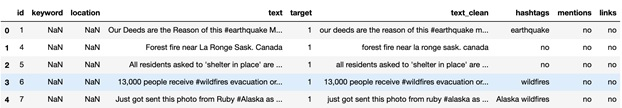
\includegraphics[scale = 0.9]{imgs/table_1.jpg}
    \label{tp:fig:location}
\end{figure}

\paragraph{Creación de features estadísticas\\}
\newline También a partir de la feature ‘text se crearon features estadísticas que nos indican:
\begin{itemize}
  \item longitud
  \item Cantidad de palabras
  \item Cantidad de palabras unicas
  \item Longitud de palabras promedio
  \item Cantidad de caracteres
  \item Cantidad de digitos
  \item Cantidad de palabras ‘stopwords’
  \item Cantidad de puntuaciones
  \item Cantidad de hashtags
  \item Cantidad de menciones
  \item Cantidad de links
  \item Cantidad de mayúsculas
  \item Y proporción de letras mayúsculas
\end{itemize}

\begin{figure}[H]
    \centering
    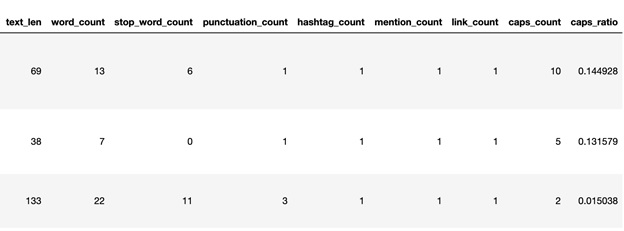
\includegraphics[scale = 0.9]{imgs/table_2.jpg}
    \label{tp:fig:location}
\end{figure}


\subsubsection{Feature ‘location’}
\paragraph{Completado de la feature\\}
\newline Se creó una nueva feature llamada ‘location\_clean’ y se completaron los valores faltantes de la feature con el valor ‘None’.


\paragraph{Limpieza de la feature\\}
Luego se procedió a unificar los valores que indicaban un mismo lugar pero estaban escritos de diferentes maneras, por ejemplo: Reino Unido es referenciado como ‘United Kingdom’, ‘UK’ y ‘Britain’, entonces se pasó todo a un único valor ‘UK’.
Solo se hizo esto con los principales valores, a los valores que no representaban mucho peso se los llamo como ‘other’.

\begin{figure}[H]
    \centering
    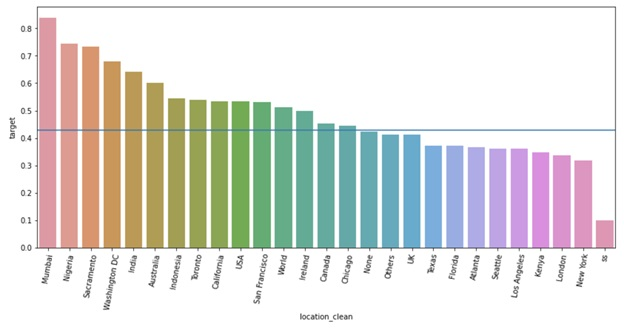
\includegraphics[scale = 0.7]{imgs/graph_1.jpg}
    \caption{Gráfico de promedio de target por ubicación}
    \label{tp:fig:equilibrium}
\end{figure}

\paragraph{Variables Categóricas\\}
Consideramos a las features keyword y location como categóricas, es por ello que se aplicó sobre ellas un target encoding utilizando la feature ‘keyword’ y la fature creada ‘location\_clean’
Antes de aplicar el target encoding sobre estas features, se llenó los NaN de la feature ‘keyword’ con la palabra ‘None’, luego se aplico el feature targeting y se crearon 2 nuevas features: ‘keyword\_target’; y ‘location\_clean\_target’.


\paragraph{Bag of Words\\}
Se aplica un bag of words sobre las features ‘links’, ‘mentions’ y ‘hashtags’.


\paragraph{TF-IDF\\}
A partir de la feature ‘text\_clean’ se aplica el algoritmo TF-IDF para crear nuevas features.
Para aplicar el algoritmo a nuestro set de datos se toman solo las palabras que aparecen mas de 10 veces, tomando unigramas y bigramas.

\paragraph{Creación de archivo csv\\}
A partir de las transformaciones creadas sobre el set de datos original, se crearon 4 archivos separados por comas nuevos tanto para train como para test:

\begin{itemize}
  \item 'train\_processed.csv'/'test\_processed.csv': contiene todas las transformaciones menos BoW y TF-IDF.
  \item 'train\_processed\_bow.csv'/'test\_processed\_bow.csv': contiene todas las transformaciones menos TF-IDF.
  \item 'train\_processed\_tf\_idf.csv'/'test\_processed\_tf\_idf.csv': contiene todas las transformaciones menos BoW.
  \item 'train\_processed\_tf\_idf\_bow.csv'/'test\_processed\_tf\_idf\_bow.csv': contiene todas las transformaciones.
\end{itemize}


%%%%%%%%%%%%%%%%%%%%%%%%%%%%%%%%%%%%%%%%%%%%%%%%%%%%%%%%%%%%%%%%%%%%%%%%%%%%%%%%%%%%%%%%%
\newpage
\subsection{Resolución Finger}
Para "calentar los dedos" y amigarse con el set de datos, python y los formatos de entrega de Kaggle se realizó una predicción muy básica sin utilizar ningún algoritmo de machine learning.
Esta predicción se basa en la siguiente idea: 

\begin{enumerate}
  \item Se toma cada tweet y se lo divide en sus palabras.
  \item Se toma cada palabra y se hace un promedio de los tweets verdadero a los que pertenece (se le llama peso de la palabra).
  \item Al tomar un tweet del set de datos lo divido en sus palabras y hago un promedio de los pesos calculados en 2 para cada palabra del tweet.
  \item Para cada tweet su predicción será el valor calculado.
\end{enumerate}

Entonces la predicción a realizar no es una clasificación sino un problema de regresión, esto es algo permitido ya que todo problema de clasificación/regresión puede ser visto como un problema de regresión/clasificación respectivamente.
Se pueden probar diferentes variantes  con el fin de mejorar el algoritmo como:

\begin{enumerate}
  \item Si el resultado de cada tweet $>$ 0.5 entonces la predicción es 1, si es $<$ 0.5 entonces la predicción es 0.
  \item Pasar todas las palabras a lowercase.
  \item Tomar los links como una misma palabra 'http' por ejemplo.
  \item Tomar la '\textbackslash n' como un separador de palabras.
  \item Se pueden eliminar las stopwords de los tweets.
  \item Quitar de las palabras todos los caracteres que no sean letras.
\end{enumerate}

\subsubsection{Primer Submit}
Se realizó un submit utilizando el promedio de las palabras para el target y se verificó que el score logrado fue 0 debido a que las predicciones esperadas son 0 o 1 y no un número real entre 0 a 1.
Entonces no podemos tomar este problema como un problema de regresión, sino que es si o si un problema de clasificación.

\subsubsection{Segundo Submit}
Con el mismo archivo que el submit anterior, se pasó el valor del target a 0 o a 1 dependiendo si el valor del promedio del peso de las palabras que forman el tweet es $<$ 0.5 o $>$ a 0.5 respectivamente.
El resultado obtenido fue de 0.77689.

Luego de notar que el problema es una clasificación y no puede ser tomado como un problema de regresión, se crearon 5 funciones para intentar mejorar la optimización:

\begin{enumerate}
  \item Si el resultado de cada tweet $>$ 0.5 entonces la predicción es 1, si es $<$ 0.5 entonces la predicción es 0.
  \item Función que pasa todas las palabras a lowercase.
  \item Función que toma a todos los links como una única palabra 'http'.
  \item Función que toma los '\textbackslash n' como separador de palabras.
  \item Función que quita todos los caracteres que no sean letras.
  \item Función que elimina todos los stopwords.
\end{enumerate}
A partir de estas modificaciones a nuestros datos se crearon las diferentes combinaciones para ver si se puede mejorar el resultado de nuestra optimización.

\subsubsection{Tercer Submit}
En este submit se llevaron todas las palabras a minúsculas (lower casing) y se hizo un nuevo submit obteniendo la puntuación de 0.78424, una importante mejora con respecto al resultado anterior y nos ubicó dentro de los primeros 1000 puestos de la competición en su momento.


\subsubsection{Cuarto Submit}
Se realizó una búsqueda de los links que contienen los tweets y se tomó a cada link como si fuera la palabra 'http'. El resultado obtenido empeora el resultado del tercer submit: 0.78332.


\subsubsection{Quinto Submit}
Se realizó un nuevo submit esta vez tomando la etiqueta '\textbackslash n' como si fuera un separador de palabras, es decir "word1\textbackslash nword2" son dos palabras diferentes word1 y word 2 separadas por el '\textbackslash n'.
El resultado obtenido fue de 0.78302.


\subsubsection{Sexto Submit}
En este submit se eliminaron las stops words del set de datos.
El resultado fue de 0.77566. Es decir, eliminar las stop words impactó negativamente en el resultado de la predicción.


\subsubsection{Séptimo Submit}
Por último se eliminan los caracteres especiales y las palabras vacías del set de datos.
El resultado obtenido fue de 0.78271.


\subsubsection{Grid Search + Cross validation}
\textbf{NOTA: el algoritmo de grid search es un algoritmo para buscar hiper parámetros y no funciones. En este apartado utilizamos el concepto de "buscar 'algo' que optimice la predicción" y no un grid search en sí mismo.\\}

Con el fin de optimizar esta idea y de aplicar estos conceptos aprendidos en clase en un problema simple, se llevó a cabo la búsqueda de la combinación de funciones que mejor resultado da en la predicción de si un tweet es de un desastre real o no.
Para cada combinación de funciones diferente se realizó un cross validation obteniendo así un puntaje del tipo F1 (idéntico al que indica en la competencia de Kaggle) y se tomó la combinación que mayor puntaje obtuvo en el cross validation.
La función de cross validation lo que hace es dividir el set de entrenamiento en 10 subsets: 9 de los subsets formarán el subset de entrenamiento y el subset restante será el subset de validación.
Se entrena el modelo con el subset de entrenamiento y se realizan predicciones sobre los datos del subset de validación. Este procedimiento se realiza 10 veces para que cada subset actúe como subset de validación y el resultado final es el promedio de los 10 resultados obtenidos.
Al realizar esta optimización se obtuvo que la combinación de funciones que mejor resultado obtuvo fue aquella formada por todas las funciones declaradas excepto la función que toma a los links como una única palabra 'http'.
Teniendo esta combinación óptima de funciones, se entrena el algoritmo con esta combinación y se realizan las predicciones sobre el set de test. Se suben estas predicciones a la competencia de Kaggle y se obtuvo un puntaje de 0.79037 que ubicó al Team en la posición 873:



\begin{figure}[H]
    \centering
    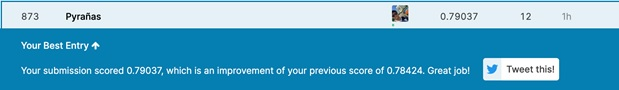
\includegraphics[scale = 0.9]{imgs/tweet_1.jpg}
    \label{tp:fig:equilibrium}
\end{figure}


Este resultado mejora bastante los resultados anteriores obtenidos aplicando las funciones de a una.


\subsubsection{Hiper-parámetro punto de corte}
A la hora de realizar la clasificación se clasifica que un tweet en real o fake según si el promedio del peso de sus palabras es mayor o igual a 0.5 o no respectivamente.
En este apartado vamos a variar desde 0 a 1, con variaciones de 0.1 para encontrar el valor de este hiper-parámetro que mejor resultados nos dé con nuestro set de datos.
Al realizar esta nueva iteración se llegó a la conclusión que el mejor resultado para el set de entrenamiento de dió aplicando las funciones que pasan el set de datos a lowercase y la que elimina del set de datos los stopwords con un punto de corte de 0.4. Al realizar el submit no se mejoró el resultado, este dió tan solo 0.77045.

Hiper-parámetro punto de corte
A la hora de realizar la clasificación se clasifica que un tweet en real o fake según si el promedio del peso de sus palabras es mayor o igual a 0.5 o no respectivamente.
En este apartado vamos a variar desde 0 a 1, con variaciones de 0.1 para encontrar el valor de este hiper-parámetro que mejor resultados nos dé con nuestro set de datos.
Al realizar esta nueva iteración se llegó a la conclusión que el mejor resultado para el set de entrenamiento de dió aplicando las funciones que pasan el set de datos a lowercase y la que elimina del set de datos los stopwords con un punto de corte de 0.4. Al realizar el submit no se mejoró el resultado, este dió tan solo 0.77045.


%%%%%%%%%%%%%%%%%%%%%%%%%%%%%%%%%%%%%%%%%%%%%%%%%%%%%%%%%%%%%%%%%%%%%%%%%%%%%%%%%%%%%%%%%
\newpage
\subsection{TensorFlow}
En esta sección se aplicará tensorflow para realizar la clasificación binaria de los tweets.


\subsubsection{Clasificación Básica}
Para realizar la primer clasificación utilizando TensorFlow se utilizan los archivos ‘train\_processed.csv’ y ‘test\_processed.csv’.
De estos archivos solo nos quedamos con las columnas ‘text\_clean’ y ‘target’, en el caso del train, ya que es el label a predecir.
Dividimos el train en dos: el texto del tweet y el target del tweet.
\paragraph{Modelo dummy\\}
En este caso se creó un tokenizador con las 3000 palabras más utilizadas de nuestro set de datos.
Se convierten los tweets en vectores en base al índice de palabras que nos da el tokenizador obteniendo a los tweets como una lista de vectores.
Creamos una matriz del tipo one-hot encoding en base a esta lista de vectores y esa es la matriz que vamos a utilizar para realizar el entrenamiendo del modelo. Este proceso se hace tanto sobre el train como sobre el test.
Luego se pasaron los labels (target) a un tipo categorical de keras, con 2 categorias posibls: 1 y 0.
Se creó un modelo sequencial de keras muy simple con las siguientes campas:
\begin{itemize}
  \item Capa densa de entrada igual al números de palabras a utilizar (3000), salida 512 y función de activación ‘relu’.
  \item Dropout de 0.2.
  \item Capa densa de salida 256 y función de activación ‘sigmoid’.
  \item Dropout de 0.2.
  \item Capa densa de salida 2 (Igual a las clases de clasificación que tengo) y función de activación ‘softmax’.
\end{itemize}
Luego se compila este modelo con función de loss ‘categorical\_crossentropy’, función de optimización ‘adam’ y obteniendo las métricas de accuracy, presición y recall.
Se entrena el modelo con batch\_size de 32, epoch de 20, validation de 0.2.
Se realizan las predicciones y se hace el submit (no se pudo realizar porque nos bloqueó Kaggle).


\paragraph{Optimizando el modelo\\}
Como bien sabemos, podemos optimizar el modelo buscando los hiperparámetros que mejor 


\subsection{Random Forest}
Es uno de los algoritmos de bagging más usados actualmente porque da buenos resultados en la mayoría de los sets de datos, también tiene la ventaja de que nos permite evaluar la importancia de los features que creamos para la toma de decisiones de los árboles.

Lo que hicimos fue aprovechar procesamiento anteriormente realizado para otros algoritmos y leer los features de los archivos train\_processed\_tf\_idf\_bow.csv para predecir, entonces utilizaremos test\_processed\_tf\_idf\_bow.csv que tiene los datos de testeo con el procesamiento realizado en los datos de entrenamiento.

Esto nos dio un resultado de 0.78210. Un poco por debajo de lo esperado, sobretodo porque la Matriz de confusión nos había dado muy buenos resultados.

Aprovechamos el Random Forest para obtener los features más importantes.



\begin{figure}[H]
    \centering
    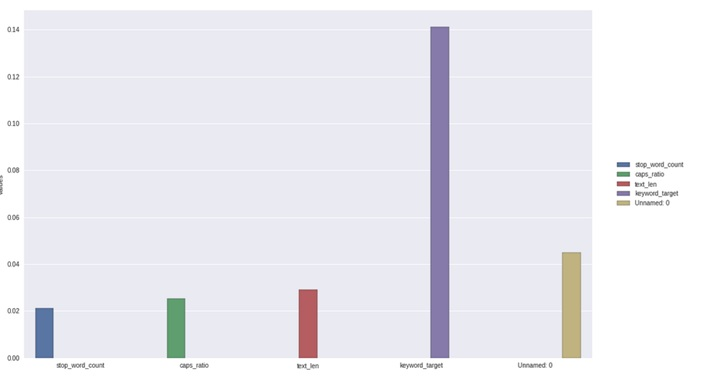
\includegraphics[scale = 0.9]{imgs/graph_2.jpg}
    \caption{Gráfico de features más importantes}
    \label{tp:fig:equilibrium}
\end{figure}

Si bien todos están por debajo de 0.15 de importancia. El feature keywork\_target parece destacar, este feature es keyword pero procesado como category. Le sigue en importancia “Unamed: 0”, en este caso esta es la etiqueta con la que quedó denominado el id de la row, así que deberemos omitirlo del análisis.
“caps\_ratio” es un feature que indica cuántas mayúsculas tiene un tuit sobre la cantidad de texto total del mismo.
“stop\_word\_count” 


\subsection{LightGBM}
Este es un algoritmo que se basa en el rendimiento. Fue diseñado para ser rápido y escalable, al igual que XGBoost está basado en árboles pero está basado en un crecimiento del árbol hacia las hojas, al contrario del XGBoost que se orienta hacia el el crecimiento en niveles (“a lo ancho”). Una ventaja es que suele ser más rápido de entrenar y consume menos memoria, pero hay que tener cuidado con el overfitting que se puede producir, esto se puede solucionar limitando el nivel de profundidad de los árboles.

El enfoque que hicimos para utilizar este algoritmo fue distinto a los anteriores. Partimos desde el set de datos utilizando solo el texto. Luego, utilizando el Universal Sentence Encoder de Google, transformamos cada texto en un encoding de igual número de columnas por cada fila.
Y con estos datos transformados entrenamos el modelo de LightGBM. En esta ocasión conseguimos un puntaje de 0.81887

\subsection{Regresion Logistica}
Con este modelo en un principio se logró un puntaje de 0.79313. El cual se pudo mejorar el puntaje agregando más estadísticas sobre la columna text\_clean. Finalmente se logró un puntaje de 0.79436


\subsection{BERT}
Este es una técnica de procesamiento de lenguaje pre entrenada desarrollada por Google que primero procesa el texto de manera tal que se consiga información sobre el contexto de cada palabra del mismo y luego se utiliza un algoritmo para realizar una predicción categórica si es necesario.
En este caso utilizamos DistilBertModel, una implementación de BERT, pre entrenada de manera tal que facilita el reconocimiento de emociones en textos.
El procesamiento que hicimos fue el siguiente: primero, solo con las primeras 2.000 filas (por problemas de RAM en el proceso siguiente), generamos un token por cada palabra del mismo. 
Luego, para que cada fila quedara con el mismo tamaño, rellenamos con “paddings” las filas que quedaran más cortas.
Después de esto indicamos al modelo de BERT qué celdas de nuestra matriz de datos correspondían a paddings y cuales  a datos a tener en cuenta.
Finalmente, con esos datos ya procesados de esta forma, realizamos una regresión logística para entrenar a nuestro modelo.
Contrariamente a lo esperado, este resultado no fue tan bueno como esperábamos, obtuvimos un puntaje de 0.78976.

\subsection{GloVe}
Es un algoritmo de aprendizaje no-supervisado para obtener representaciones de vectores de palabras significativas. El entrenamiento se genera sobre la estadística de co-ocurrencia entre un par de palabras. Este método permite observar patrones lineales en el espacio vector-palabra.
En este caso la implementación es sencilla por lo que el resultado del testeo es bajo (0.68). Comparando con otros notebooks en kaggle, se observa que luego de una análisis extenso que incluye limpieza y corrección ortográfica de datos.
Otro dato importante es que el algoritmo sale a relucir con textos mas largos ya que al poseer múltiples tuplas se tiene una aproximación más realista.

%%%%%%%%%%%%%%%%%%%%%%%%%%%%%%%%%%%%%%%%%%%%%%%%%%%%%%%%%%%%%%%%%%%%%%%%%%%%%%%%%%%%%%%%%
\newpage
\section{Conclusión}
Fue muy importante realizar los primeros submits con la predicción según el peso de las palabras de los tweets ya que al realizarlas se comprobó que el valor del target tiene que ser 1 o 0 y no un valor real entre 0 y 1. Esto quiere decir que la competencia es una competencia de clasificación y no de regresión.
También notamos en el Finger como al buscar la combinación de funciones que mejor resultado dan en un cross validation la puntuación mejora considerablemente, por lo que el proceso de optimización es un proceso muy importante para cualquier algoritmo de machine learning.



%%%%%%%%%%%%%%%%%%%%%%%%%%%%%%%%%%%%%%%%%%%%%%%%%%%%%%%%%%%%%%%%%%%%%%%%%%%%%%%%%%%%%%%%%
\newpage
\section{Referencias}
\begin{itemize}
  \item 75.06, 95.58 Organización de Datos - Apunte del curso - Luis Argerich, Natalia Golmar, Damián Martinelli, Martín Ramos Mejía, Juan Andrés Laura.
  \item Videos del canal de youtube.com de 7506 - Organización de Datos (\url{https://www.youtube.com/channel/UCCG5Fs18xdJlNstK1sbKxuA})
  \item \url{http://apuntes-r.blogspot.com/2014/12/bagging-para-mejorar-un-modelo.html}
\end{itemize}

\end{document}